% Chapter X

\chapter{DSMC WITH SPIN - EHRENFEST} % Chapter title

\label{ch:dsmcehr} % For referencing the chapter elsewhere, use \autoref{ch:dsmcehr} 

To include the effects of Majorana spin flips in our DSMC simulations we will obviously have to develop some semiclassical method \ie simulate the positions of the atoms classically using the DSMC method and simulate the internal state of the atom with a quantum mechanical approach.
One such approach would be to use the Ehrenfest theorem \cite{Ehrenfest1927} to calculate the average force applied to an atom based on its current internal state (I have given a brief pseudo-code in listing \ref{lst:Ehrenfest}).
Using this method we would evolve the internal state of the atom using the Schr\"odinger equation then, using the internal state of the atom, we can calculate the expectation value of the force to use in evolving the position of the atom.

Unfortunately this technique is not a viable solution, as we will demonstrate in this chapter.
While we are able to capture some of the interesting physics (usually short term) of the Majorana spin flip using the Ehrenfest approach, it just fails over long simulation periods.


%----------------------------------------------------------------------------------------

\section{Simulating Schr\"odinger Equation}

To make use of the proposed Ehrenfest method (EM) we need to be able to accurate solve the Sch\"odinger equation.
Some of the more straight forward approached might be to apply a finite difference technique directly to the pde, however these methods are not generally conservative \cite{?}.
In fact the techniques that are considered more stable generally have some non-physical numerical dissipation as a results of the approximations made \cite{?} (or even show?).

The approach we have employed here, and in chapter \ref{ch:dsmcmcwf}, is to make use of the unitary time evolution operator \cite{?}.
The main benefit of this approach is, as the name suggests, the operator is unitary and hence inherently conserves probability.
The unitary time evolution operator is defined as follows
\begin{equation}
    \widehat{U}(t_0,t_0+\Delta t) = \exp\left[-\frac{\imath}{\hbar}\int_{t_0}^{t_0+\Delta t} \widehat{H}(t)\,dt \right]. \label{eq:timeEvolution}
\end{equation}
That is for a time dependant Hamiltonian we can evolve the state of our wavefunction, $\vert \psi \rangle$, through a moment of time $\Delta t$, through the application of the time evolution operator, $\widehat{U}$,
\begin{equation*}
    \ket{ \psi (t_0+\Delta t) } = \widehat{U}(t_0,t_0+\Delta t) \ket{ \psi (t_0) }.
\end{equation*}
This method is especially useful for our two level system as we can explicitly derive an expression for the $2\times2$ matrix form of $\widehat{U}$.
Recall from section \ref{sec:intromag} that the Hamiltonian for a magnetic moment in a magnetic field is given by
\begin{equation*}
    \widehat{H} = -\hat{\boldsymbol{\mu}} \cdot \mathbf{B},
\end{equation*}
which can be expressed in matrix form as
\begin{equation*}
    \widehat{H} = \frac{1}{2}g_s\mu_B \begin{bmatrix} B_z & B_x - \imath B_y \\
                                                      B_x + \imath B_y & -B_z \end{bmatrix}.                                          
\end{equation*}
In general the magnetic field components are functions of position, which, for the atoms is a function of time.
For a general magnetic field we do not know explicitly what the time dependance will be and so we will not be able to explicitly integrate the Hamiltonian as required by equation \eqref{eq:timeEvolution}.
\marginpar{Make a side note about higher order integration.}
So we will have to make the assumption that our time steps are very small, $\Delta t \ll 1$, so that over the time step the Hamiltonian remains relatively constant.
In this limit we have, $\int\widehat{H}\,dt = \widehat{H}\Delta t$, so that the time evolution operator becomes
\begin{align}
    \widehat{U}(t_0,t_0+\Delta t) &= \exp\left[  -\imath\frac{g_s\mu_B\Delta t}{2 \hbar} \begin{bmatrix} B_z & B_x - \imath B_y \\
                                                      B_x + \imath B_y & -B_z \end{bmatrix} \right],\\
                &= \begin{bmatrix} \cos\theta - \imath n_z \sin\theta & -\left(n_y+\imath n_x\right)\sin\theta \\
                                   \left(n_y-\imath n_x\right)\sin\theta & \cos\theta + \imath n_z \sin\theta\end{bmatrix}, 
\end{align}
where $\theta = g_s \mu_B \Delta t \vert \mathbf{B} \vert / 2\hbar$ and $n_k = B_k / \vert \mathbf{B} \vert$ are the directional components of the magnetic field normal vector.
This simple closed form expression makes it very easy to implement the unitary evolution operator method numerically.

%------------------------------------------------

\section{Schr\"odinger Simulations}

To test out this technique lets just numerically solve the original Majorana problem \eqref{eq:Majprob}.
In figure \ref{fig:majprob} I have simulated two scenarios: a spin flip (figs \ref{fig:labframeFlip}, \ref{fig:rotframeFlip}) and a not flip (figs \ref{fig:labframeNoFlip}, \ref{fig:rotframeNoFlip}).
Each scenario is plotted in two seperate refernce frames: the laboratory frame and the co-rotating frame.
The laboratory frame is the frame in which the spin up direction is aligned with the $z$-axis, the co-rotating frame is the frame in which the spin up direction is aligned with the magnetic field.
\marginpar{We find the spin up and spin down components in the co-rotating frame by projecting onto the "local" magnetic field. We do this using the projection operator, $ \ket{\phi_{\uparrow,\downarrow}} = \widehat{P}_{\uparrow,\downarrow} \ket{\Psi}$, where the projection operator is given by $\widehat{P} = ??$.}
The laboratory frame is the frame in which the differential equation is set, however in this frame it can become a little confusing about wether a particular spin state is flipped our not.
In both of the simulations the direction of the magnetic field changes at $t=0$, so the orientation of the spin up direction in the lab frame also changes.
In the co-rotating frame it is always clear which state is the spin up state.

\begin{figure}
\hspace{-6em}
\makebox[1.8\linewidth][l]{%
\centering
\subfloat[Lab frame flip, $B_t=1\times10^{-7}$]{\label{fig:labframeFlip}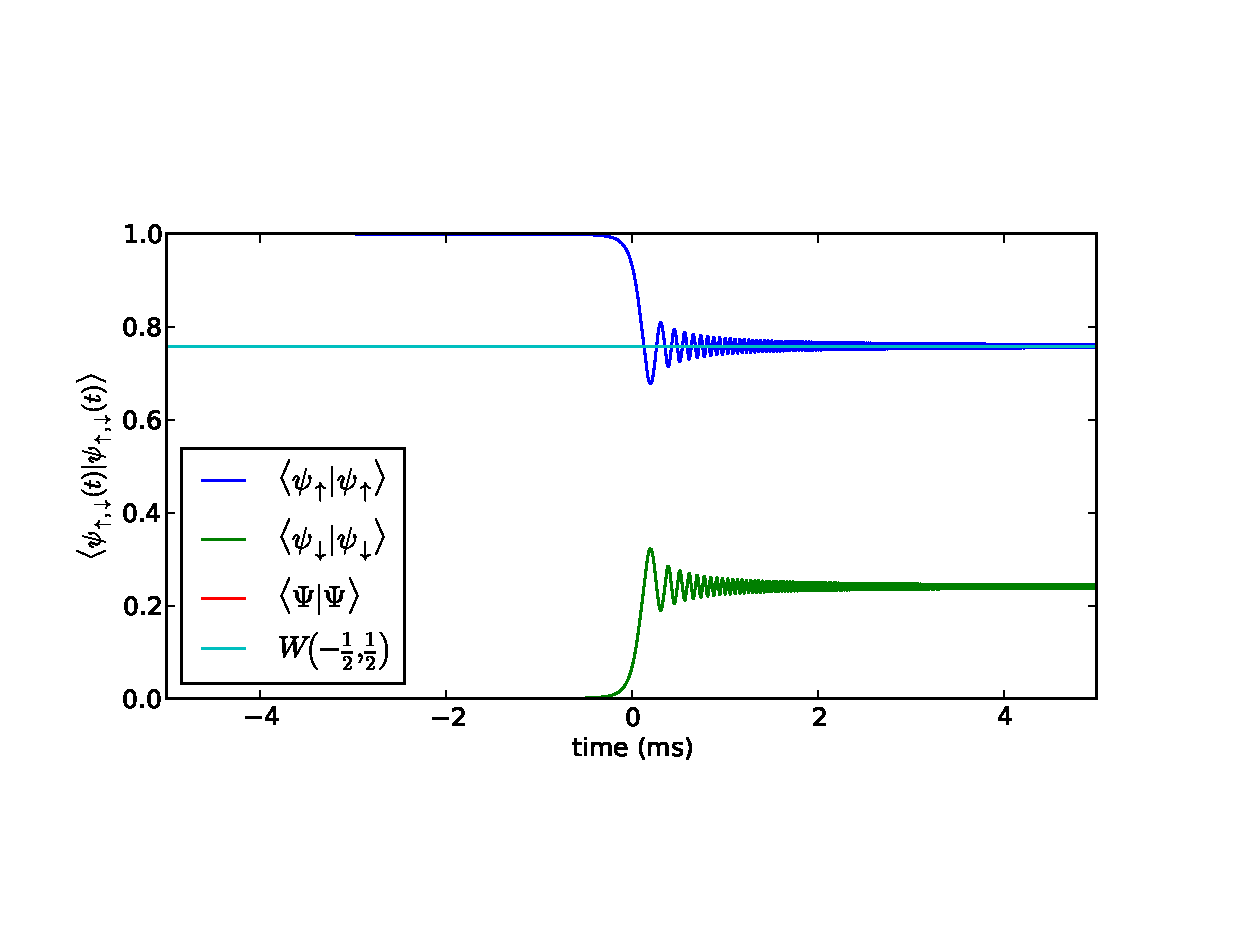
\includegraphics[width=0.75\textwidth]{gfx/Ehrenfest/labframeFlip}}\quad
\subfloat[Rotating frame flip]{\label{fig:rotframeFlip}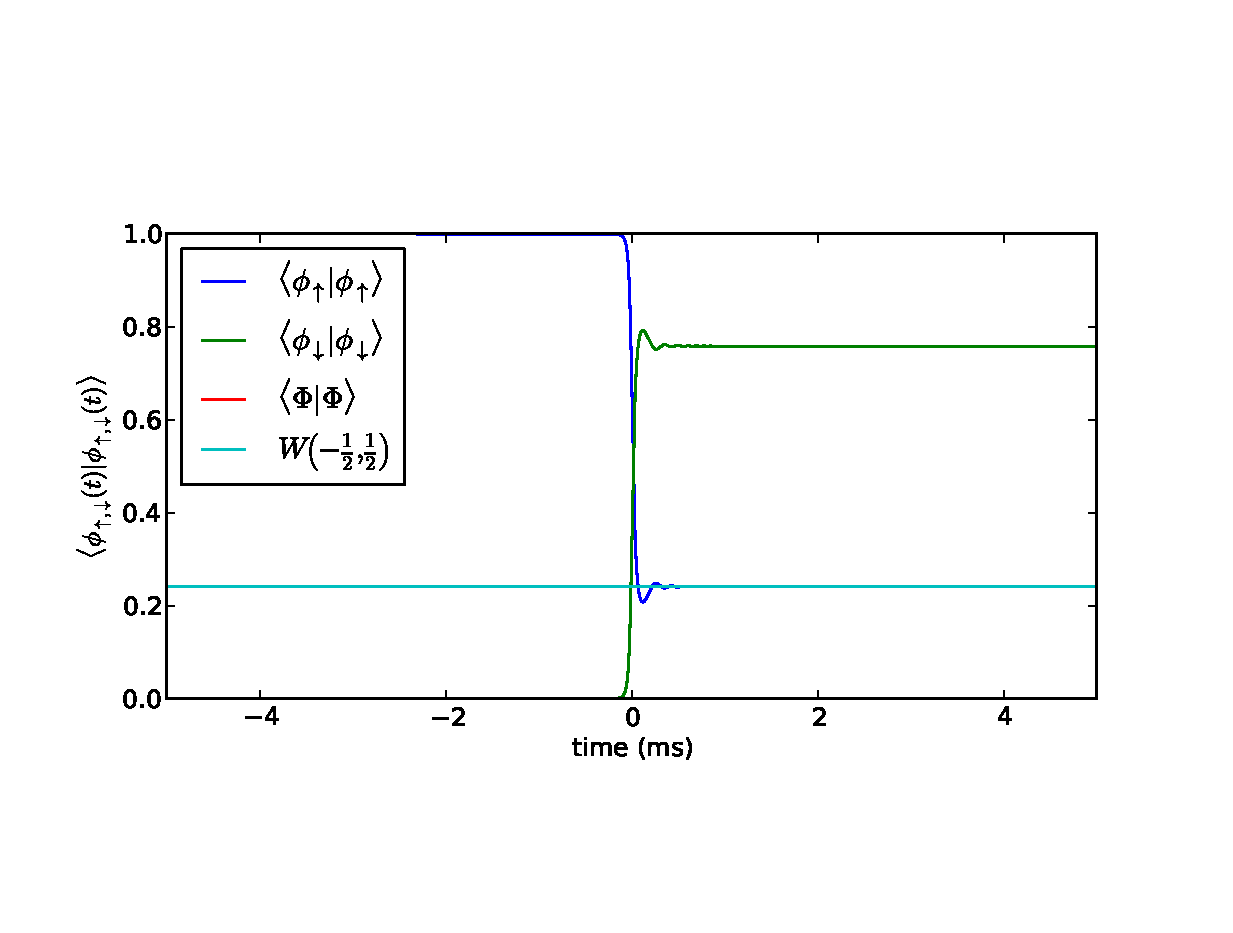
\includegraphics[width=0.75\textwidth]{gfx/Ehrenfest/rotframeFlip}}
}\\\_
\hspace{-6em}
\makebox[1.8\linewidth][l]{%
\centering
\subfloat[Lab frame no flip, $B_t=2\times10^{-7}$]{\label{fig:labframeNoFlip}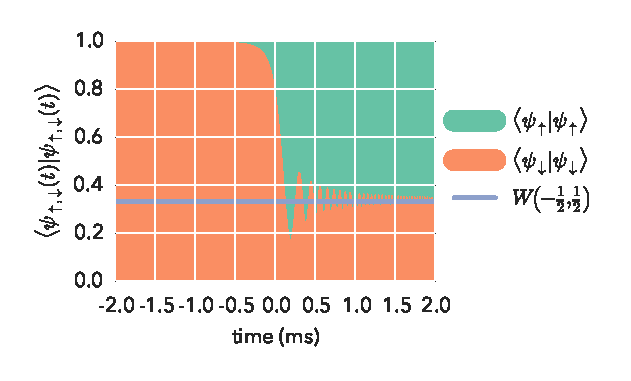
\includegraphics[width=0.75\textwidth]{gfx/Ehrenfest/labframeNoFlip}}\quad
\subfloat[Rotating frame no flip]{\label{fig:rotframeNoFlip}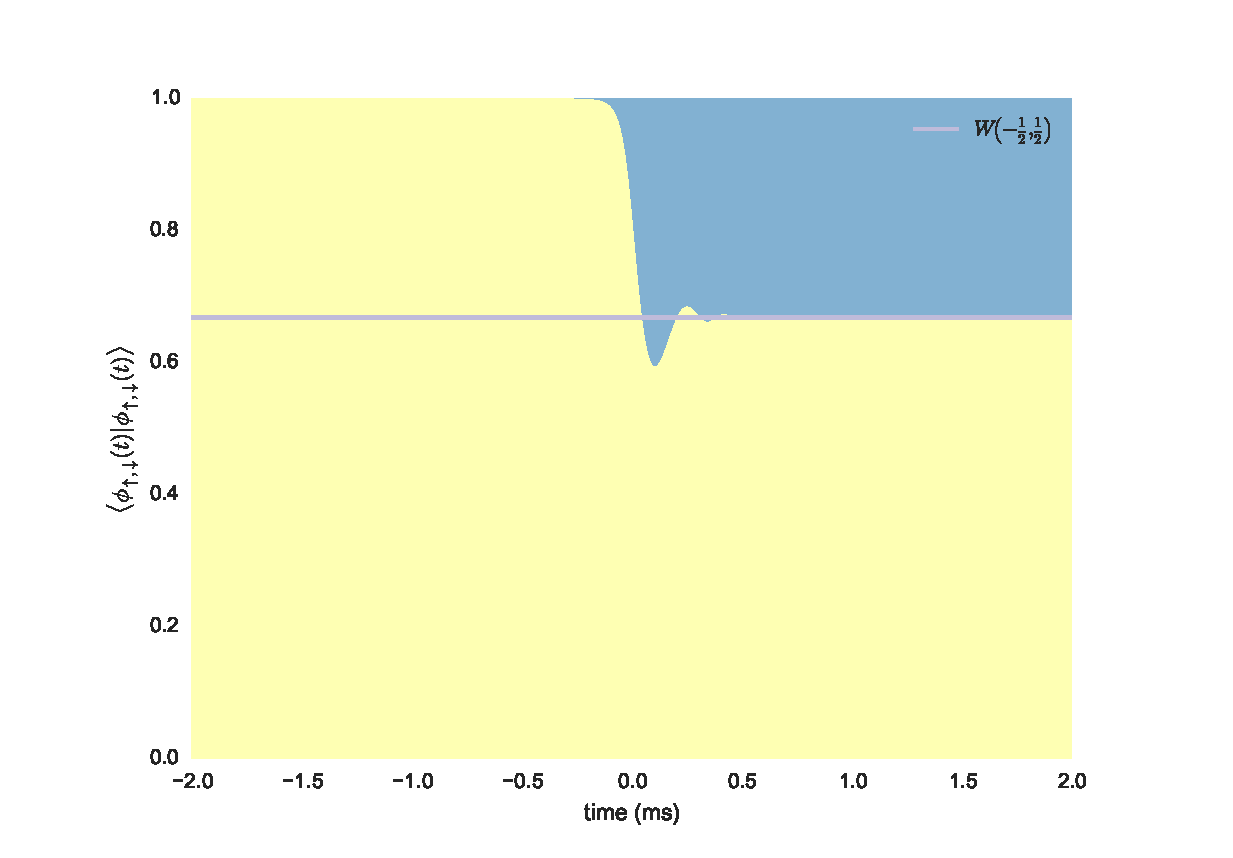
\includegraphics[width=0.75\textwidth]{gfx/Ehrenfest/rotframeNoFlip}}
}
\caption{Simulating the no majorana spin flip }\label{fig:majprob}
\end{figure}

Figures \ref{fig:labframeFlip} and \ref{fig:rotframeFlip} both illustrate a Majorana spin flip.
In this simulation we used the magnetic field $\mathbf{B}=(0.1,0.0,2500t)\,\mathrm{mT}$, and began at $t=-15\,\mathrm{ms}$ where the population in the spin component in the lab frame is less than $10^6$ (although we have plotted a smaller time window in figure \ref{fig:majprob}).
We can see the distinct different between the behaviour of the spin populations in the two different reference frames.
The initial wavefunction was chosen such that the population of the spin up component in the lab frame was 1.
Figure \ref{fig:rotframeFlip} clearly displays a change in the most probable state, whereas in figure \ref{fig:labframeFlip} it is not so clear.
Again this is because in the lab frame the spin up direction changes at $t=0$ when the sign of the $z$ component of the magnetic field moves from negative to positive.
Figures \ref{fig:labframeNoFlip} and \ref{fig:rotframeNoFlip} results from a simulation with $\mathbf{B}=(0.2,0.0,2500t)\,\mathrm{mT}$.
In these plots we see the converse behaviour in the state populations, indicating that no spin flip has occurred.

For both simulations we have used a time step of $\Delta t = 1\,\mu\mathrm{s}$.
This may seem overkill given the rate of change of the magnetic field can be characterised by $\tau_B=\vert\mathbf{B}\vert / \partial_t\vert\mathbf{B}\vert = 15\,\mathrm{ms}$ at the beginning of the simulation.
However there is another time scale that must be considered in a simulation like this, that is the period of a Larmor precession, $T_L = 2\pi\hbar / g_s \mu_B \vert\mathbf{B}\vert = 3.81\,\mu\mathrm{s}$ at the begining of the simulation.
While we do not expect the spin to precess for the first half of the simulation when it is completely aligned with the magnetic field, it is the period close to the field minimum and beyond that will experience Larmor precession.
In fact the wiggles after the spin flip occur at the Larmor precision frequency.
For example, look at one period of oscillation around $t=0.3\,\mathrm{ms}$, here the Larmor precession period will be, $T_L=0.19\,\mathrm{ms}$, exactly as simulated (**MAKE INSET IN FIGURE TO SHOW LARMOR PRECESSION RATE**).

\marginpar{The astute reader may be confused by line 4 of the pseudo-code in listing \ref{lst:Ehrenfest}.
The appearance of the $n+1^\mathrm{th}$ velocity when calculating the $n+1^\mathrm{th}$ position is not how one might implement the standard Euler integration method. 
Here we have used an implementation of the Symplectic Euler method \cite{??}, which has better energy conserving properties than the standard forward Euler.
This technique still has the same order accuracy with time, and introduces no added computational complexity, yet we gain some extra stability in the total energy of the atom.}

%------------------------------------------------

\section{Single Atom Spin Flips}

Confident in our ability to accurately simulate the Schr\"odinger equation, in our regime of interest, we may begin to apply the Ehrenfest method to simulating spin flips of real atoms.
The first step is to first see wether or not we can simulate the spin flip of a single atom.
I have given a pseudo-code example for a single time step of the Ehrenfest algorithm in listing \ref{lst:Ehrenfest}\footnote{Note in listing \ref{lst:Ehrenfest} that we have denoted the discrete approximation to a continuous variable as, $g_n \approx g(t_n)$.}.
\begin{lstlisting}[float,caption=Psuedo-code algorithm for a single Ehrenfest method time step, mathescape,label= lst:Ehrenfest,stepnumber=1]
Calculate force using current spin state: $\mathbf{F}_n = \bra{\Psi_n}\widehat{\mathbf{F}}_n\ket{\Psi_n}$.
Evolve wavefunction using time evolution operator: $\ket{\Psi_{n+1}} = \widehat{U}_n \ket{\Psi_{n}}$.
Evolve velocity using the average force: $\mathbf{v}_{n+1} = \mathbf{v}_n + \mathbf{F}_n \Delta t / m$.
Evolve position using the new velocity: $\mathbf{x}_{n+1} = \mathbf{x}_n + \mathbf{v}_{n+1} \Delta t$.
\end{lstlisting}

\begin{figure}
\hspace{-8em}
\makebox[1.8\linewidth][l]{%
\centering
\subfloat[Co-rotating frame spins]{\label{fig:ehrenfestSpin}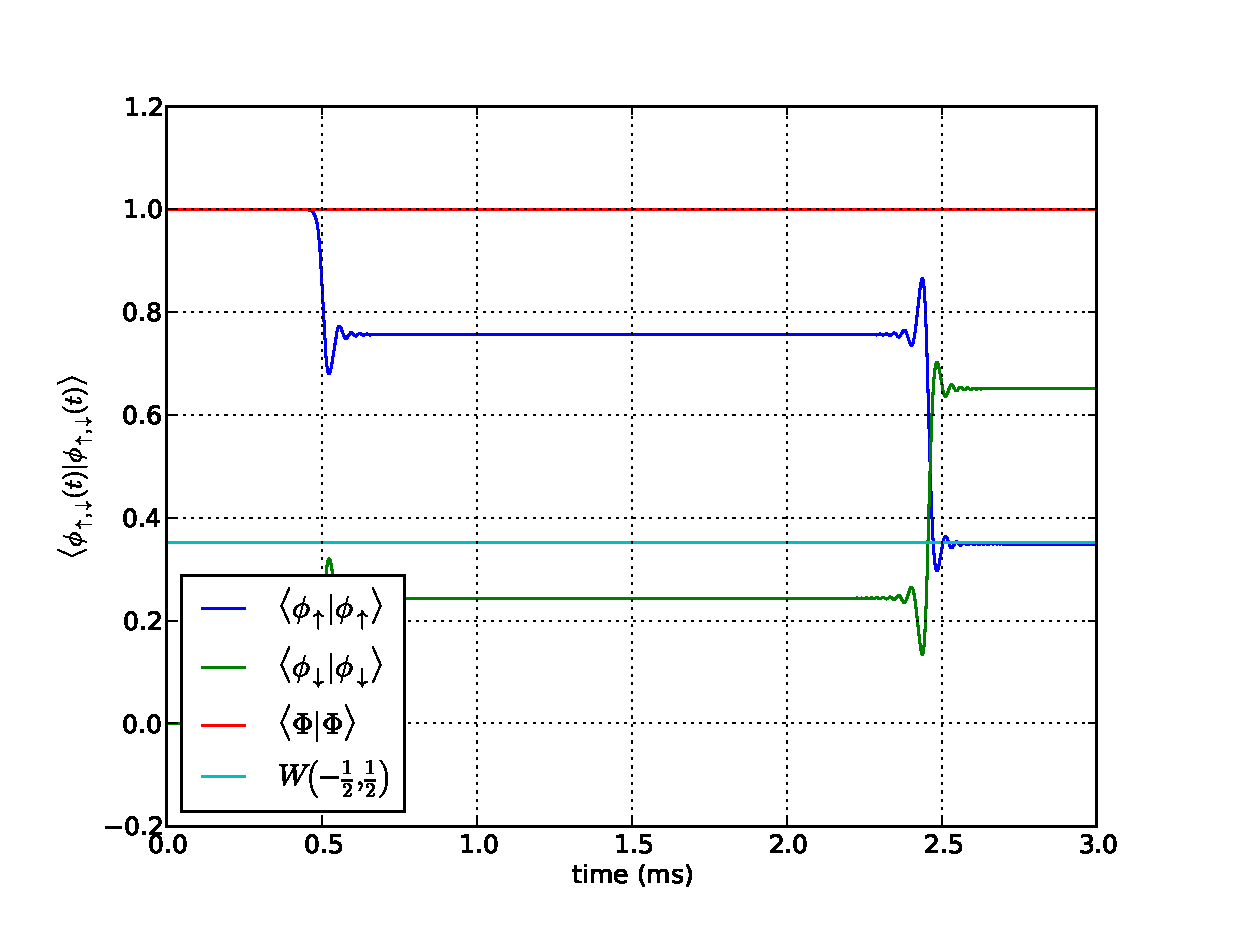
\includegraphics[width=0.525\textwidth]{gfx/Ehrenfest/ehrenfestSpin}}\quad
\subfloat[Position and velocity]{\label{fig:ehrenfestPos}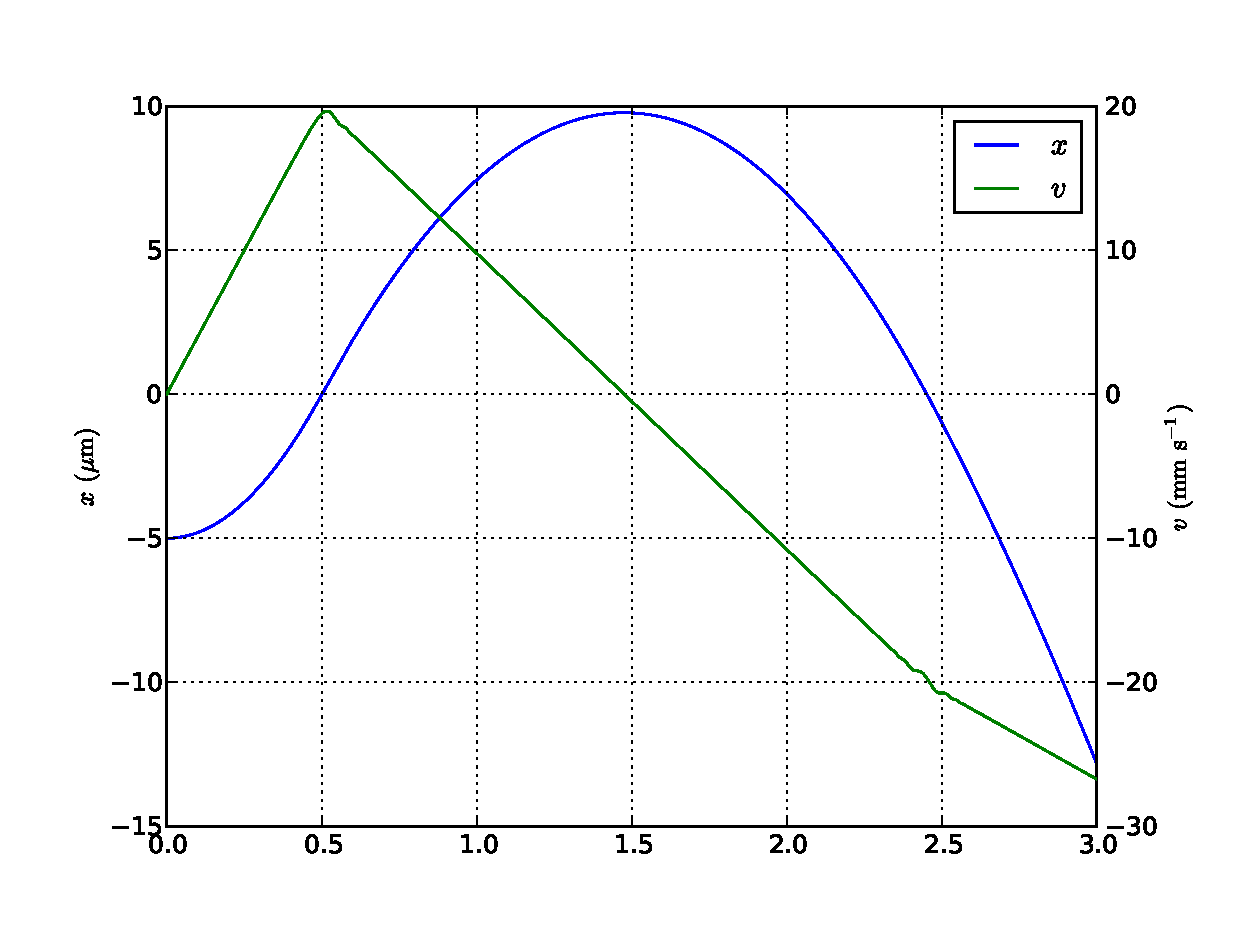
\includegraphics[width=0.525\textwidth]{gfx/Ehrenfest/ehrenfestPos}}\quad
\subfloat[Energy]{\label{fig:ehrenfestEnergy}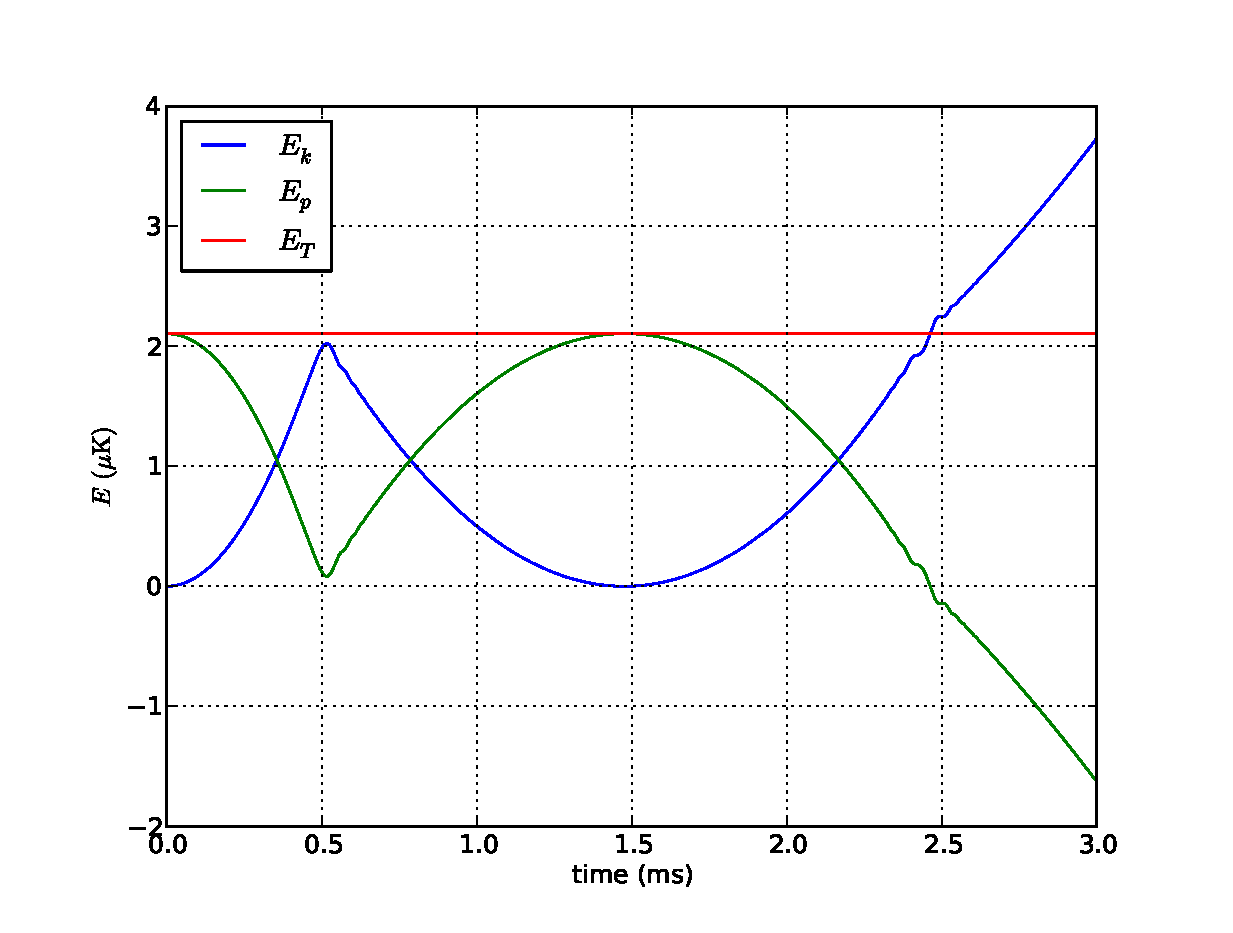
\includegraphics[width=0.525\textwidth]{gfx/Ehrenfest/ehrenfestEnergy}}%
}
\caption{No flip and flip in the same simulation.}\label{fig:ehrenfestFlip}
\end{figure}

Figure \ref{fig:ehrenfestFlip} shows the results from one such simulation.
This simulation was of a rubidium 87 atom the began at $x=-5\,\mu\mathrm{m}$ with a zero initial velocity.
Again the initial wavefunction was chosen so that it would be completely spin up in the co-rotating frame.
The magnetic field was given by $\mathbf{B} = (B_x,0,B_z'z)$, with $B_z=1\,\mu\mathrm{T}$ and $B_z'=2.5\,\mathrm{Tm}^{-1}$\footnote{I am aware that this magnetic field does not satisfy Maxwell's equations, but it serves as a nice example and more closely aligns with the field considered by Majorana.}.
This is a fabulous example of how well the Ehrenfest method can work.
Figure \ref{fig:ehrenfestSpin} displays how well the spin populations are simulated.
Again they agree with the predictions of the Majorana formula and the total probability is conserved.
\marginpar{Say how I can still use the Majorana formula here. $c =v(t=0) B_z'$.}
In figure \ref{fig:ehrenfestPos} I have plotted the position and velocity of the atom as it moves through time.
We can see how the atom remains trapped after the first partial flip and is then completely ejected from the trapped once it has flipped.
Finally figure \ref{fig:ehrenfestEnergy} shows how the total energy of the atom is conserved throughout the simulation (even after is has flipped).
So things seem to be working quite well, but earlier I alluded to the fact that the Ehrenfest method is not suitable to this kind of problem, so what is wrong?
I will let you stew on this few a few sections while we investigate the behaviour of a full gas simulation.

%----------------------------------------------------------------------------------------

\section{Full Gas Simulations}

Content

%------------------------------------------------

\subsection{Ioffe Pritchard Trap}

Content

%------------------------------------------------

\subsection{Quadrupole Trap}

Content